% ASCEND 1.5.0 Layer 2.2 annotated 3D midpoint-iPVDR figure.
% The heatmap is raster; all arrows, mathematical labels and panels remain
% exact TikZ vectors in the compiled document.

\begin{figure}[htbp]
\centering
\begin{tikzpicture}[
  samplearrow/.style={-Latex, line width=1.15pt, draw=blue!75!black},
  valleyarrow/.style={-Latex, line width=1.15pt, draw=orange!90!black},
  neighbour/.style={<->, >=Latex, line width=1.45pt, draw=teal!75!black},
  formula/.style={rounded corners=2pt, draw=black!50, fill=white,
                  fill opacity=0.88, text opacity=1, inner sep=4pt,
                  font=\small},
  result/.style={rounded corners=2pt, draw=teal!75!black, very thick,
                 fill=white, fill opacity=0.90, text opacity=1,
                 inner sep=5pt, font=\small}
]

\node[anchor=south west, inner sep=0] (image) at (0,0)
  {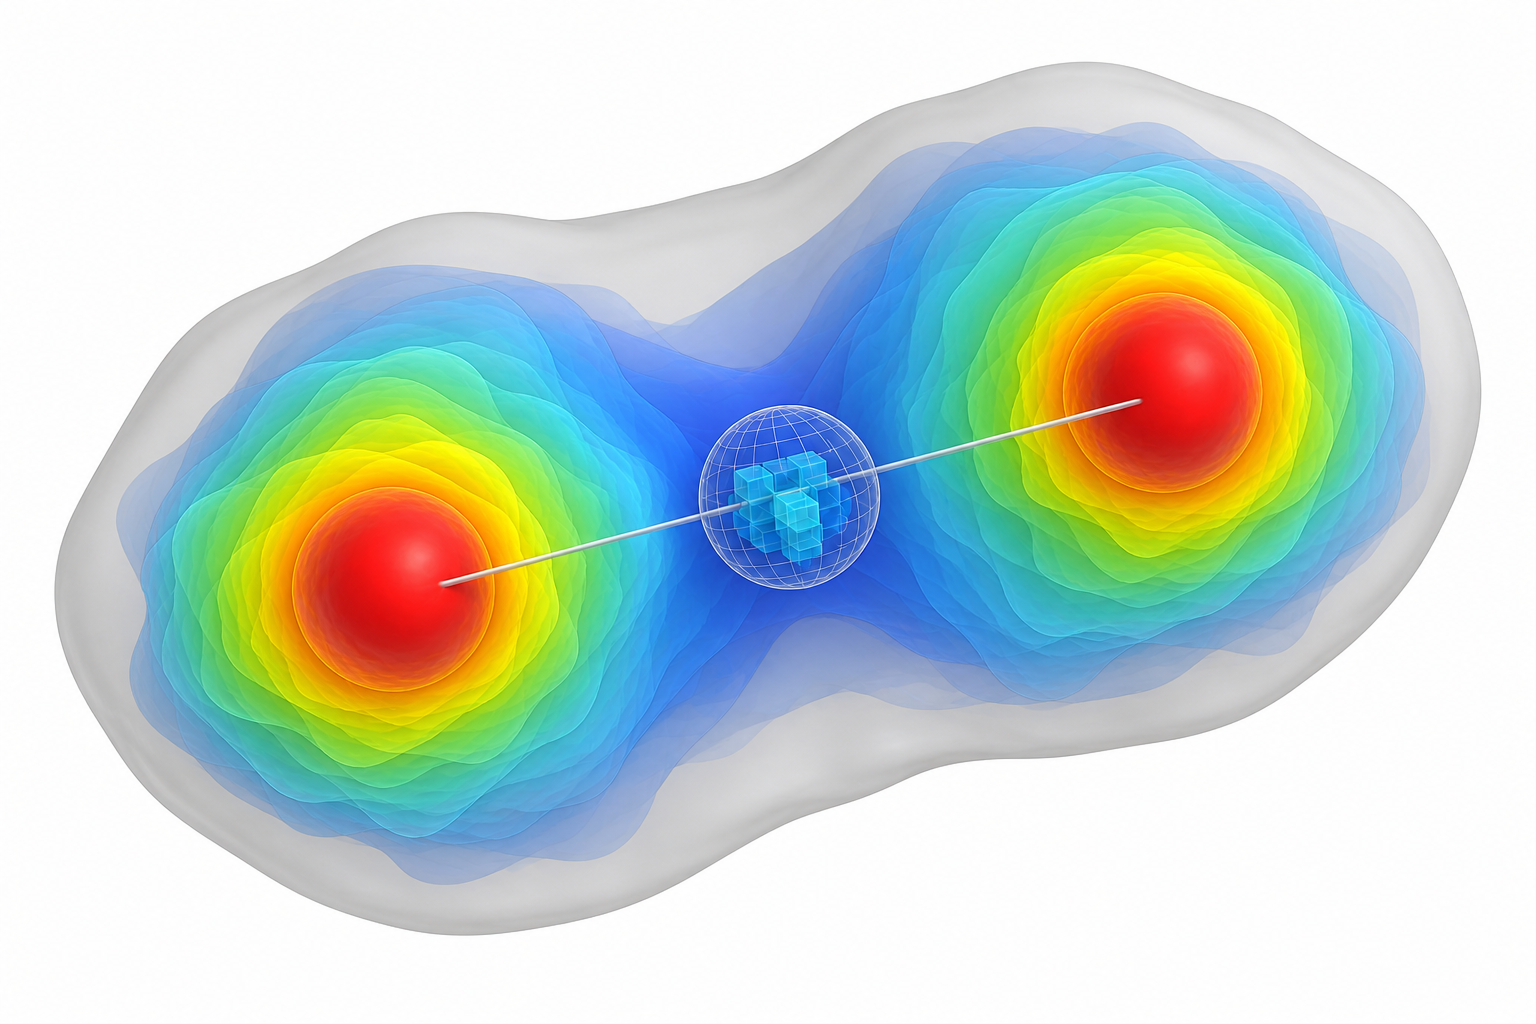
\includegraphics[width=0.96\linewidth]{docs/figures/ascend-layer22-ipvdr-3d-heatmap-clean-white.png}};

% Normalised image coordinates: (0,0) is lower left and (1,1) is upper right.
\begin{scope}[x={(image.south east)},y={(image.north west)}]

% Native vertex D50 samples.
\node[formula] (leftdose) at (0.14,0.76)
  {$D_{50\%}\!\left(\mathrm{VTV}_{H,i}\right)$};
\draw[samplearrow] (leftdose.south east) -- (0.235,0.445);

\node[formula] (rightdose) at (0.86,0.82)
  {$D_{50\%}\!\left(\mathrm{VTV}_{H,j}\right)$};
\draw[samplearrow] (rightdose.south west) -- (0.756,0.625);

% Native midpoint-sphere median sample and its fixed sampling radius.
\node[formula, draw=orange!90!black] (valleydose) at (0.52,0.255)
  {$\displaystyle
    \begin{gathered}
    D_{\mathrm{valley},ij}=D_{50\%}\!\left(S_{ij}\right)\\[-2pt]
    r=3\,\mathrm{mm}
    \end{gathered}$};
\draw[valleyarrow] (valleydose.north) -- (0.510,0.515);

% Midpoint and exact centroid-to-centroid nearest-neighbour vector.
\draw[neighbour] (0.235,0.445) -- (0.756,0.625);
\node[formula, draw=teal!75!black] at (0.505,0.705)
  {$\displaystyle
    \begin{gathered}
    \mathbf{m}_{ij}=\frac{\mathbf{c}_{i}+\mathbf{c}_{j}}{2}\\[-1pt]
    d_{ij}=\left\lVert\mathbf{c}_{j}-\mathbf{c}_{i}\right\rVert_{2}
    \end{gathered}$};

% Local peak from the two endpoint median doses.
\node[formula, draw=blue!75!black, font=\scriptsize] at (0.275,0.105)
  {$\displaystyle
    D_{\mathrm{peak},ij}
    =\frac{
      D_{50\%}\!\left(\mathrm{VTV}_{H,i}\right)
      +D_{50\%}\!\left(\mathrm{VTV}_{H,j}\right)
    }{2}$};

% Edge-local ratio assembled from the sampled peak and valley terms.
\node[result] at (0.755,0.105)
  {$\displaystyle
    \mathrm{iPVDR}_{ij}
    =\frac{D_{\mathrm{peak},ij}}{D_{\mathrm{valley},ij}}$};

\end{scope}
\end{tikzpicture}
\caption{Conceptual three-dimensional representation of the ASCEND Layer 2.2
midpoint-iPVDR calculation. Blue arrows identify the two endpoint vertex
$D_{50\%}$ samples, the orange arrow identifies the median dose sampled from
the 3~mm midpoint sphere, and the double-headed vector shows the physical
nearest-neighbour connection. This explanatory illustration is not patient
data and is not geometrically scaled.}
\label{fig:ascend-ipvdr-3d-annotated}
\end{figure}
